\documentclass[oneside, 11pt]{book}

%\usepackage[italian]{babel}
%\usepackage[latin1]{inputenc}
\usepackage[pdftex]{graphicx} \pdfcompresslevel=9
\usepackage{amsmath}

\graphicspath{{./images/}}

\begin{document}

\begin{titlepage}
\vspace*{0.5\textwidth}
\begin{center}
{\Huge \textbf{RTI Viewer User Manual}}
\\
\vspace{1.0cm}
Version 0.1
\end{center}

\end{titlepage}

\tableofcontents

\chapter{Introduction}
In this document we present the main features of RTI Viewer. Especially we describe how the user can interact with the GUI and the effects produced by his actions.

RTI Viewer is a tool to diplay images produced with reflection transformation techniques. The tool supports several image formats: Polynomial Texture Maps (PTM), Adaptive PTM (APTM), Hemispherical Harmonics Maps (HSH) and an universal format that encodes all previous images (URTI).

The tool permits to open an image or from a local hard disk or from a remote server and to set some parameters of rendering such as the zoom factor, the sub-image to show in the browser, the light direction and only for the PTM format the rendering mode to enhance the perception of shapes and details.

\chapter{GUI}
RTI Viewer is composed by several widgets that permit to the user to interact using mouse and keyboard. As shown in Figure \ref{fig:rtiviewer}, these widgets are:
\begin{itemize}
\item the \emph{Browser} to display the RTI image;
\item the \emph{Toolbar};
\item the \emph{Light Control} to select the light direction;
\item the \emph{Rendering Dialog} to select the rendering mode to apply to the RTI image;
\item the \emph{Navigator} to pan and zoom the RTI image.
\end{itemize}

Some information about the open image (path to the file, image size and image format) is shown between the Rendering Dialog and the Navigator.

\begin{figure}[htbp!]
  \centering
  
\includegraphics[width=\textwidth]{rtiviewer}
  \caption{RTI Viewer GUI.}
  \label{fig:rtiviewer}
\end{figure}

\section{Browser}
The Browser permits to display the output of the rendering of the RTI image (see Figure \ref{fig:browser}). The user can use the mouse to pan the image and to set the light direction, and the keyboard for the zoom operations. Especially the dragging with the left button of the mouse permits to move the sub-image in the current view of the browser, while the dragging with the right button permits to move the light direction. The double-click with the left button moves the center of the browser in the point of the click and performs a zoom in operation. Finally the keyboard shortcuts CTRL + `+' and e CTRL + `-' permit respectively the zoom in and the zoom out operations.

\begin{figure}[htbp!]
  \centering
  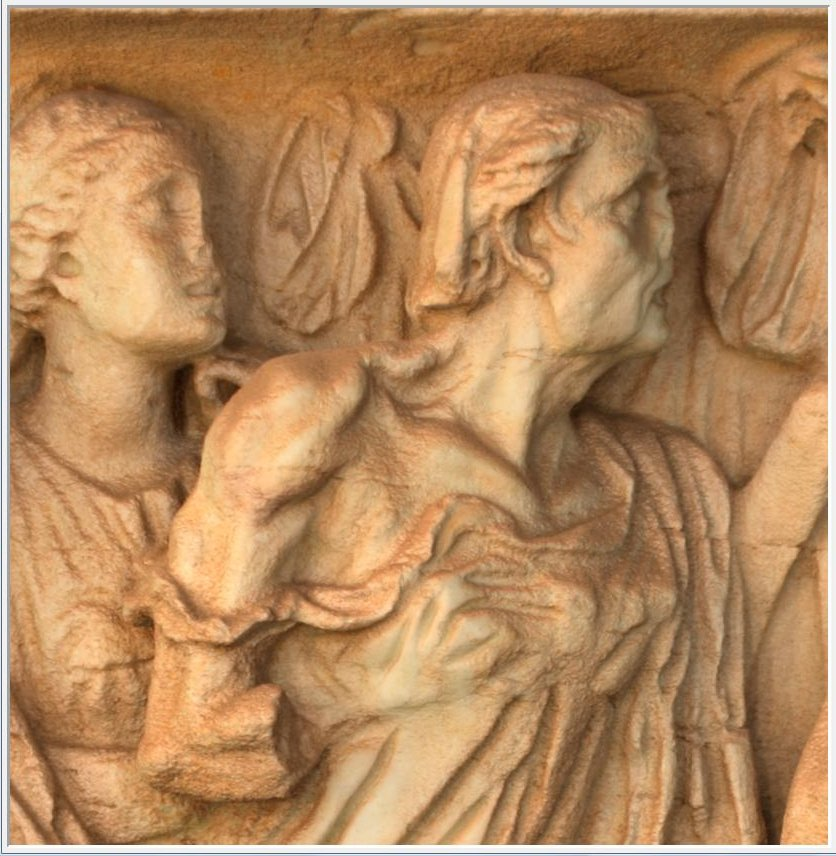
\includegraphics[width=0.7\textwidth]{browser}
  \caption{Browser.}
  \label{fig:browser}
\end{figure}

\section{Toolbar}
The buttons in the toolbar permit, from left to right in Figure \ref{fig:toolbar}:
\begin{itemize}
\item to open an image from a local hard disk;
\item to open an image published on a remote server (the user must insert the URL of the image);
\item to save a snapshot of the image displayed in current view of the browser;
\item to modify the settings of the application. The user can only modify the size of the browser (see Figure \ref{fig:appSettings});
\item to show a window with infomation about the tool.  
\end{itemize}

\begin{figure}[hb!]
  \centering
  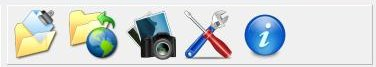
\includegraphics[width=0.5\textwidth]{toolbar}
  \caption{Toolbar.}
  \label{fig:toolbar}
\end{figure}

\begin{figure}[hb]
  \centering
  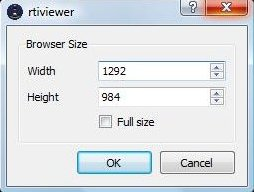
\includegraphics[width=0.45\textwidth]{app_settings}
  \caption{Window to set the application settings.}
  \label{fig:appSettings}
\end{figure}


\section{Light Control}
The Light Control permits to the user to select the light direction to use in the rendering of the RTI image by means of the left button of the mouse. The current light direction is shown by the highlight on the sphere (see Figure \ref{fig:lightcontrol}).

\begin{figure}[hbt]
  \centering
  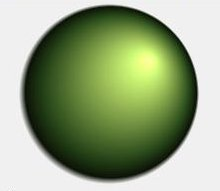
\includegraphics[width=0.4\textwidth]{lightcontrol}
  \caption{Light Control.}
  \label{fig:lightcontrol}
\end{figure}

\section{Rendering Dialog}
The Rendering Dialog permits to select the rendering mode to apply to RTI image. For each mode the dialog displays the widget to set some characteristic parameters. The list of available rendering modes is function of the type of image. In the current version of the tool, only the PTM have other modes in addition to the standard rendering.

The available modes for the PTM are:
\begin{itemize}
\item Diffuse Gain;
\item Specular Enhancement;
\item Luminance Unsharp Masking;
\item Image Unsharp Masking;
\item Normal Enhancement (or Normal Unsharp Masking);
\item Coefficient Enhancement (or Coefficient Unsharp Masking);
\item Detail Enhancement (or Static Multi-light Detail Enhancement);
\item Dynamic Detail Enhancement (or Dynamic Multi-light Detail Enhancement).
\end{itemize}

All methods permit to vary in real-time the light direction except the Detail Enhancement that creates a static image. A more detailed description of the methods can be founded in \ref{} and \ref{}.

\subsection{Diffuse Gain}
Diffuse Gain enhances the perception of the surface shape of the object. The user can modify a gain factor to fix the amount of the enhancement (see Figure \ref{fig:diffuseGain}).

\begin{figure}[hbt]
  \centering
  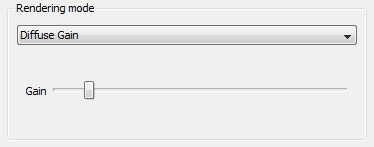
\includegraphics[width=0.5\textwidth]{diffuse_gain}
  \caption{Parameters of Diffuse Gain.}
  \label{fig:diffuseGain}
\end{figure}

\subsection{Specular Enhancement}
Specular Enhancement adds a specular effect to the surface of the object. The method uses the following lighting model:
\begin{equation}
    I = (k_{d} (\vec{L} \cdot \vec{N}) + k_{s} (\vec{H} \cdot \vec{N})^{n})
\end{equation}
where $\vec{L}$ is the light vector, $\vec{N}$ is the normal and $\vec{H}$ is the halfway vector between the the light vector and the viewer. The user can modify the gain factor to fix the amount of the enhancement, the diffusive constant $k_{d}$, the specular constant $k_{s}$ and the specular exponent $n$ (see Figure \ref{fig:specularEnh}).

\begin{figure}[hbt]
  \centering
  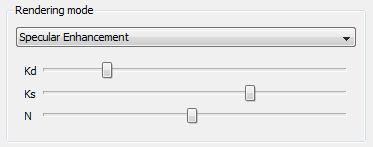
\includegraphics[width=0.5\textwidth]{specular_enh}
  \caption{Parameters of Specular Enhancement.}
  \label{fig:specularEnh}
\end{figure}

\subsection{Luminance Unsharp Masking}
Luminance Unsharp Masking applies the classic unsharp masking to the luminance component of LRGB PTM. It can not be applied to the RGB PTM. The user can modify a gain factor to fix the amount of the enhancement (see Figure \ref{fig:luminanceUM}).

\begin{figure}[hbt]
  \centering
  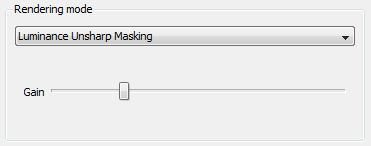
\includegraphics[width=0.5\textwidth]{luminance_um}
  \caption{Parameters of Luminance Unsharp Masking.}
  \label{fig:luminanceUM}
\end{figure}

\subsection{Image Unsharp Masking}
Image Unsharp Masking applies the classic unsharp masking to the Y channel of the color space YUV. The user can modify a gain factor to fix the amount of the enhancement (see Figure \ref{fig:imageUM}).

\begin{figure}[hbt]
  \centering
  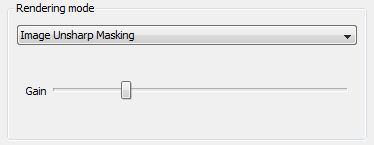
\includegraphics[width=0.5\textwidth]{image_um}
  \caption{Parameters of Image Unsharp Masking.}
  \label{fig:imageUM}
\end{figure}

\subsection{Normal Enhancement}
Normal Enhancement applies the classic unsharp masking to the surface normals. The method uses the following lighting model:
\begin{equation}
    I = \vec{N} \cdot \vec{L} + k_{a}
\end{equation}
where $\vec{N}$ is the normal, $\vec{L}$ is the light vector and $k_{a}$ is a term to preserve the amount of light received by the surface through inter-reflection and ambient light. The user can modify a gain factor to fix the amount of the enhancement and the term $k_{a}$ (see Figure \ref{fig:normalEnh}).

\begin{figure}[hbt]
  \centering
  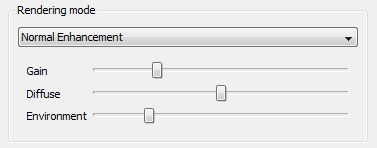
\includegraphics[width=0.5\textwidth]{normal_enh}
  \caption{Parameters of Normal Enhancement.}
  \label{fig:normalEnh}
\end{figure}

\subsection{Coefficient Enhancement}
Coefficient Enhancement applies the classic unsharp masking to the coefficients of the polynomial of the PTM. The user can modify a gain factor to fix the amount of the enhancement (see Figure \ref{fig:coeffEnh}).

\begin{figure}[hbt]
  \centering
  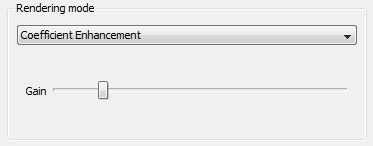
\includegraphics[width=0.5\textwidth]{coeff_enh}
  \caption{Parameters of Coefficient Enhancement.}
  \label{fig:coeffEnh}
\end{figure}

\subsection{Detail Enhancement}
Detail Enhancement produces automatically an high-contrast, well-illuminated static image for stand-alone presentation, high-quality printing, or similar purposes. The method has several advanced settings that require a good knowledge of its basis algorithm. 

\subsection{Dynamic Detail Enhancement}
Dynamic Detail Enhancement adapts locally the current light direction to improve the perception of the details on the surface. The user can modify the size of the tile and the maximum offset in degree from the current light direction (see Figure \ref{fig:dynDetail}). The method has several advanced settings that require a good knowledge of its basis algorithm.

\begin{figure}[hbt]
  \centering
  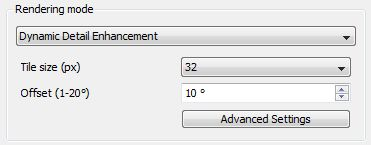
\includegraphics[width=0.5\textwidth]{dyn_detail_enh}
  \caption{Parameters of Dynamic Detail Enhancement.}
  \label{fig:dynDetail}
\end{figure}


\section{Navigator}
The Navigator permits to the user to move and resize the sub-image in the current view of the browser. The sub-image is shown in the widget with a red rectangle. The user can move the rectangle with the left button of the mouse or can resize the rectangle with the dragging of the triangle in the bottom-right corner (see Figure \ref{fig:navigator}).

\begin{figure}[hbt]
  \centering
  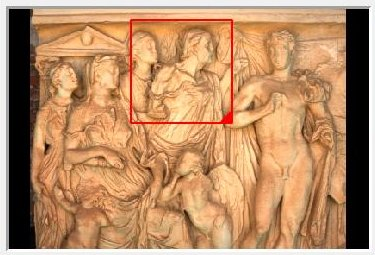
\includegraphics[width=0.5\textwidth]{navigator}
  \caption{Navigator.}
  \label{fig:navigator}
\end{figure}

\end{document} 